% ——————————————————————————————————————————————————————————————————
%Экспериментальные настройки для https://www.nngroup.com/articles/design-thinking/. TODO: выпилить нумерацию в оглавлении, попробовать *ещё_раз* подобрать менее контрастную антикву с поддержкой textbf
% ——————————————————————————————————————————————————————————————————
\documentclass[12pt]{article}

\usepackage{import}
\import{preamble/}{preamble}
\graphicspath{{img/}}

\begin{document}
\title{Основы дизайн-мышления}

{\noindent\sffamily\huge\bfseries Основы дизайн-мышления\par}
\par
\vspace{0.8em}
\articleauthor{design-thinking-author.jpg}{\href{https://www.nngroup.com/articles/author/sarah-gibbons/}{Сара Гиббонс}}{31 июля 2016 г. \(\cdot\) Пересмотрено 15 июля 2026 г.}


% ——————————————————————————————————————————————————————————————————
%Далее и ниже идут костыли для жирного начертания. Да простят меня все те, кто будет когда-либо читать исходник
% ——————————————————————————————————————————————————————————————————
\begin{leftbar}
	\large{{\fontseries{b}\selectfont Кратко:} Дизайн-мышление~"--- это процесс, ориентированный на пользователя, который помогает командам понимать потребности, генерировать идеи, тестировать решения и способствовать инновациям.}
\end{leftbar}


\vspace{0.8em}
{\noindent{\large\fontseries{b}\selectfont Содержание\par}}
\vspace{-0.8em}
	\begin{leftbar}
		\vspace{-12pt}
		\tableofcontents
	\end{leftbar}

\section{Определение дизайн-мышления}

Дизайн-мышление~"--- это {\fontseries{b}\selectfont методология}\footnote{В оригинале автор использует термин ideology~"--- «идеология», но в русском языке это слово имеет явно выраженный социологический оттенок.}, подкрепляемая соответствующим процессом. Для полного понимания нужно разобраться в обоих. 

\begin{leftbar} 
	{\fontseries{b}\selectfont Дизайн-мышление} утверждает, что прикладной, ориентированный на пользователя подход к решению проблем, ведёт к инновациям, а инновации помогают выделиться на рынке и получить конкурентное преимущество. Этот прикладной, ориентированный на пользователя подход, определяется {\fontseries{b}\selectfont дизайн-процессом} и состоит из шести различных этапов, о которых будет рассказано ниже.
\end{leftbar}

\section{Процесс}

Фреймворк дизайн-мышления состоит из трёх шагов:   
\begin{enumerate*}[label=\arabic*)]
	\item understand~"--- понять;
	\item explore~"--- изучить;
	\item materialize~"--- воплотить.
\end{enumerate*}
Внутри этих крупных разделов выделяют~\hyperref[pic:poster]{шесть этапов:}
\begin{enumerate*}[label=\arabic*)]
	\item empathize~"--- эмпатия (сопереживание);
	\item define~"--- анализ и~определение проблемы;
	\item ideate~"--- генерация идей;
	\item prototype~"--- прототипирование;
	\item test~"--- тестирование;
	\item implement~"--- внедрение.
\end{enumerate*}

\begin{figure}[H]
	\centering
	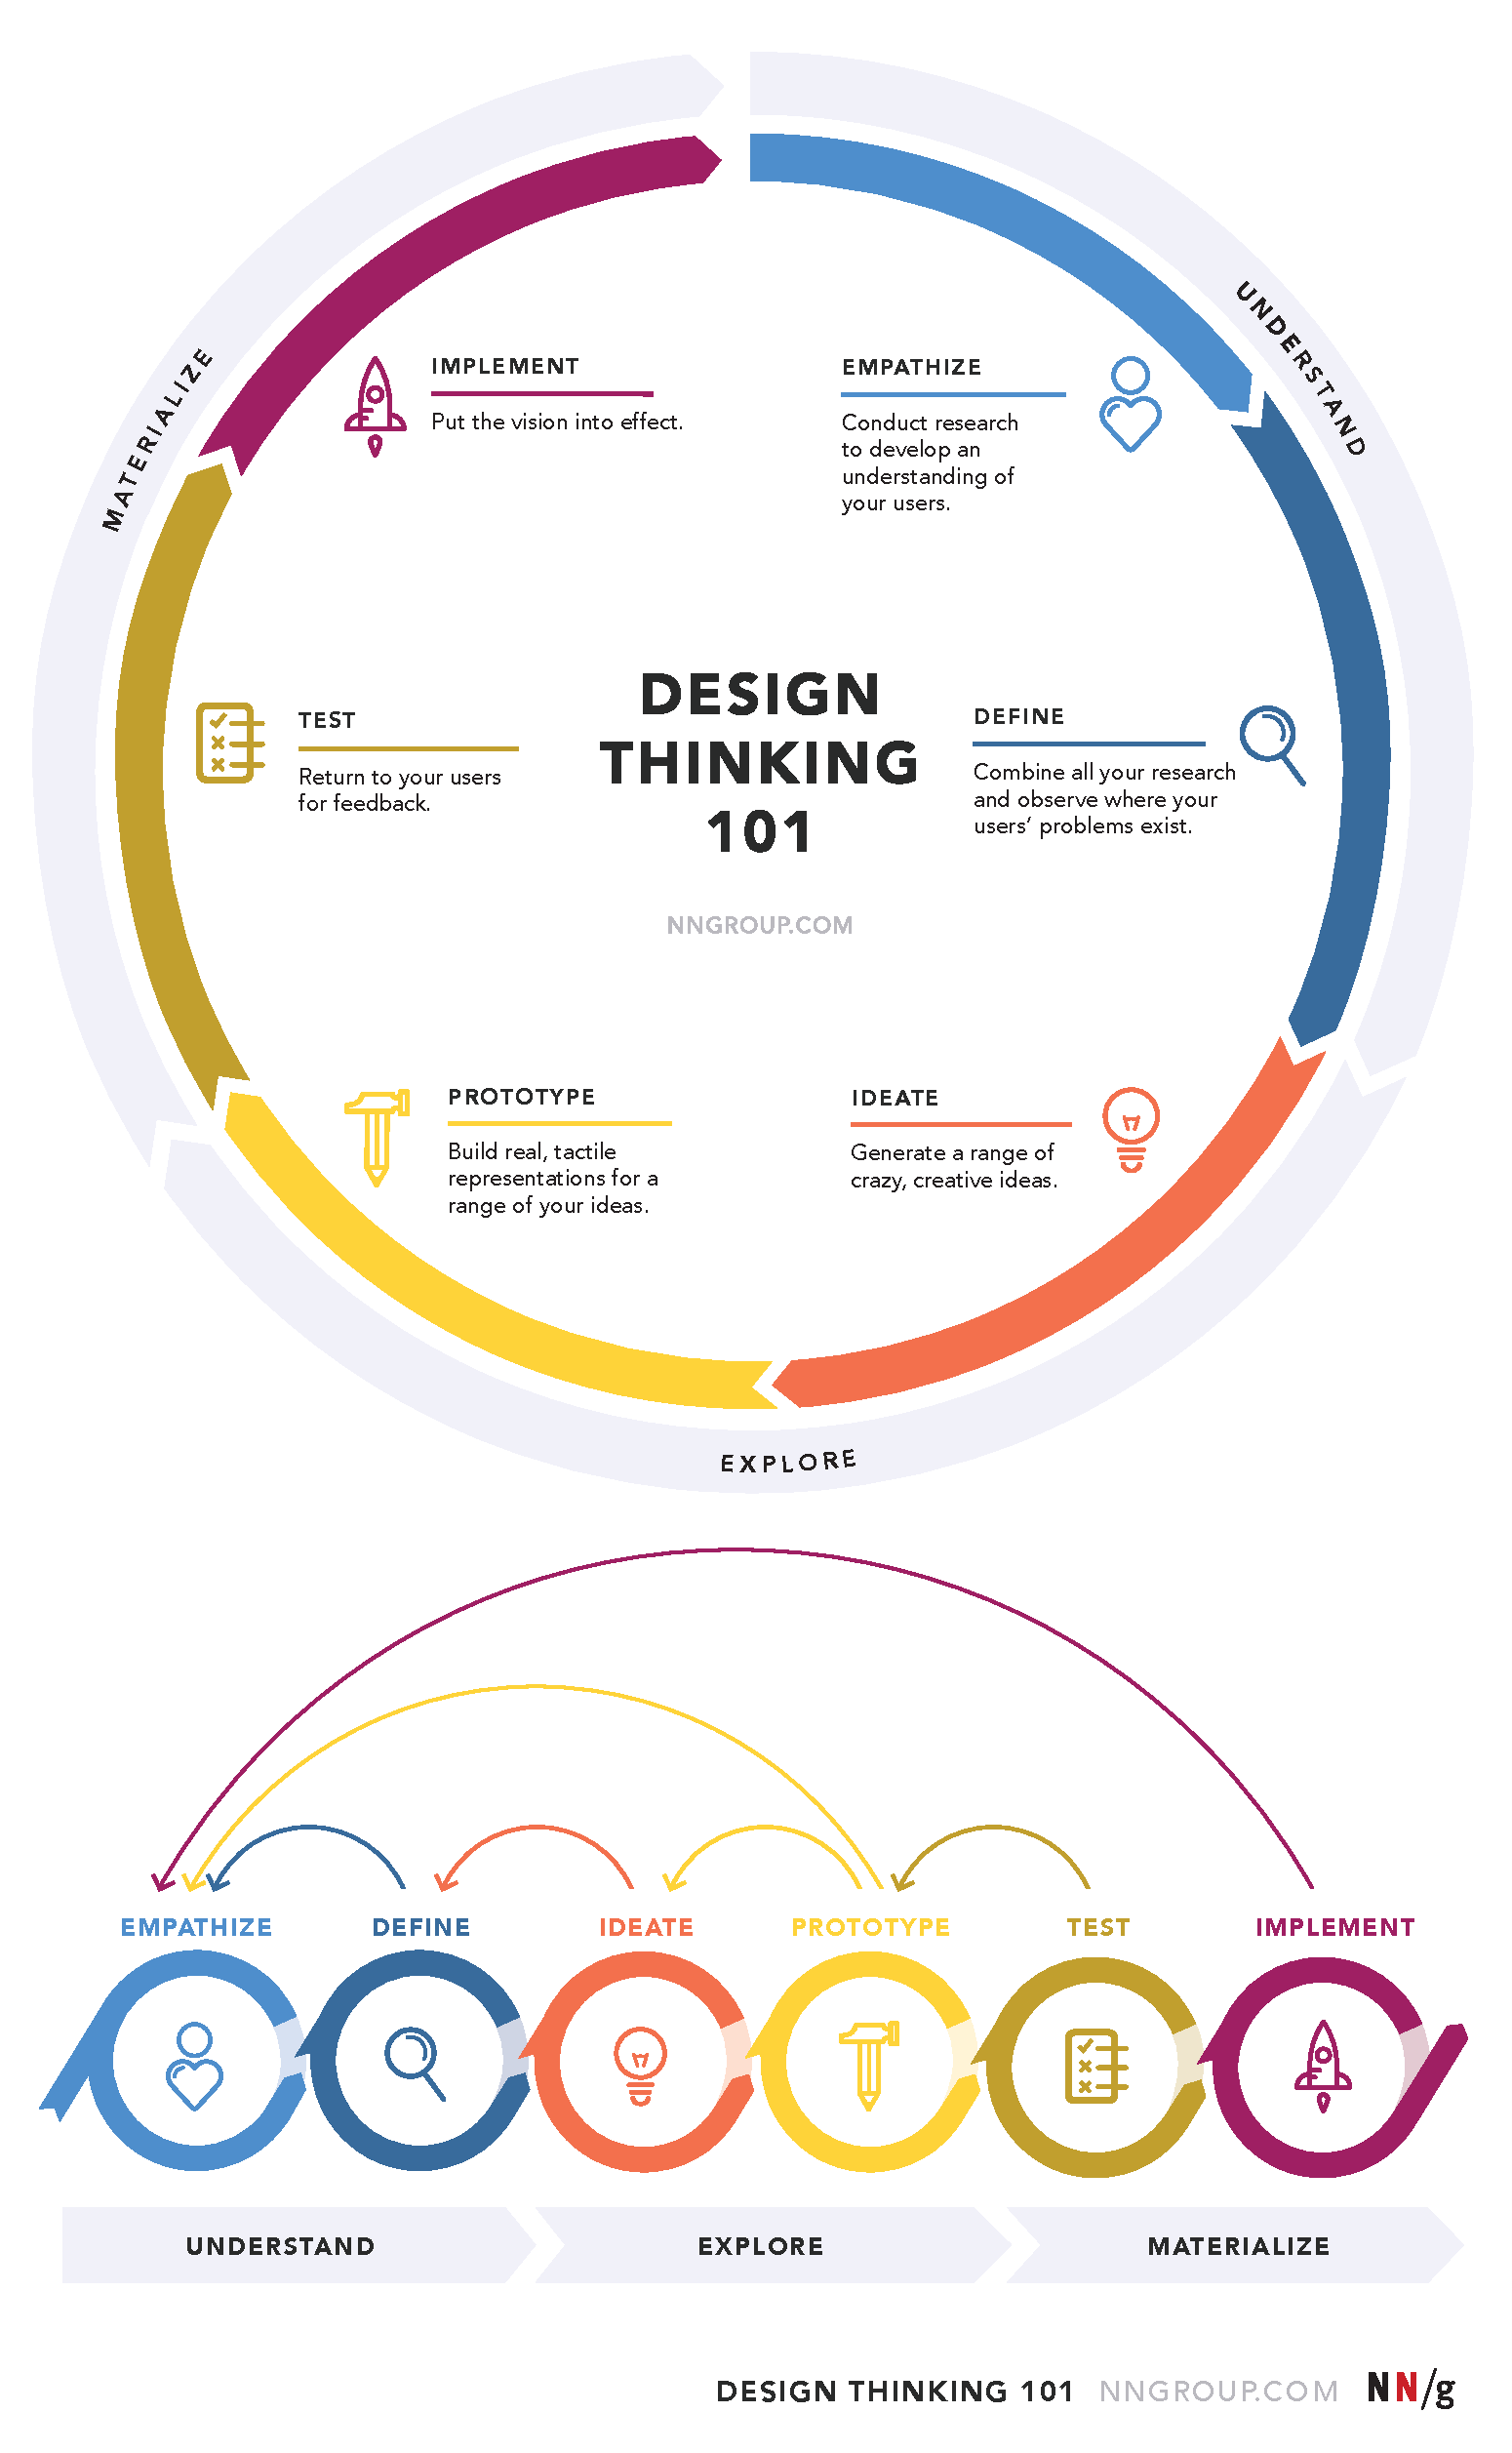
\includegraphics[width=\textwidth, height=0.85\textheight, keepaspectratio]{Design-thinking-101-NNG.pdf}
	\par
	\vspace{2em}
	\mbox{{\fontfamily{far}\selectfont\href{https://media.nngroup.com/media/articles/attachments/Design-thinking-101-NNG.pdf}{Design Thinking (PDF)}}}
	\label{pic:poster}
\end{figure}


\section{Зачем~"--- в чём преимущество}
\section{Гибкость~"--- адаптация под ваши потебности}
\section{Масштабируемость~"--- мыслите шире}
\section{История дизайн-мышления}

\end{document}